
\chapter{Pengenalan Elixir}

\section{Elixir}

Elixir adalah bahasa pemrograman fungsional yang dirancang untuk membangun aplikasi yang scalable dan maintainable. Dikembangkan oleh José Valim, Elixir berjalan di atas Erlang Virtual Machine (BEAM) dan memanfaatkan keunggulan teknologi Erlang untuk manajemen proses dan concurrent programming. Bahasa ini sering digunakan dalam pengembangan aplikasi berskala besar, seperti sistem web yang memerlukan performa tinggi dan kemampuan untuk menangani banyak koneksi secara bersamaan.

\subsection{Mengapa Elixir Ada}

Elixir diciptakan untuk mengatasi beberapa keterbatasan yang ada pada bahasa pemrograman lain, khususnya dalam konteks aplikasi yang memerlukan skalabilitas tinggi dan keandalan yang kuat. Berikut adalah beberapa alasan utama mengapa Elixir dikembangkan:

\begin{itemize}
	\item \textbf{Mengatasi Keterbatasan Bahasa Lain:} José Valim, pengembang Elixir, merasa bahwa bahasa pemrograman yang ada saat itu tidak sepenuhnya memenuhi kebutuhan aplikasi modern yang memerlukan concurrency, fault tolerance, dan scalability. Elixir dirancang untuk mengatasi kekurangan ini dengan memanfaatkan kekuatan Erlang.
	
	\item \textbf{Memanfaatkan Infrastruktur Erlang:} Elixir dibangun di atas Erlang Virtual Machine (BEAM), yang sudah terbukti andal dalam menangani aplikasi dengan banyak koneksi secara bersamaan dan dalam situasi yang memerlukan toleransi kesalahan. Dengan memanfaatkan BEAM, Elixir mewarisi kekuatan concurrency dan fault tolerance dari Erlang, tetapi dengan sintaksis yang lebih modern dan fitur tambahan.
	
	\item \textbf{Produktivitas Pengembang:} Elixir dirancang untuk meningkatkan produktivitas pengembang dengan menyediakan fitur-fitur seperti metaprogramming dan sintaksis yang bersih dan intuitif. Ini memungkinkan pengembang untuk menulis kode yang lebih mudah dibaca dan dikelola, serta mempercepat pengembangan aplikasi.
	
	\item \textbf{Pengembangan Aplikasi Web Modern:} Seiring dengan meningkatnya kebutuhan untuk aplikasi web yang real-time dan dinamis, Elixir menawarkan solusi yang efektif dengan framework seperti Phoenix. Phoenix mendukung real-time communication dan pengembangan aplikasi web yang responsif, menjadikannya pilihan yang menarik untuk pengembangan web modern.
	
	\item \textbf{Kebutuhan Scalability dan Fault Tolerance:} Dalam dunia teknologi yang terus berkembang, aplikasi perlu mampu menanggapi peningkatan beban kerja dan potensi kegagalan sistem. Elixir memberikan alat dan struktur untuk membangun aplikasi yang dapat dengan mudah diskalakan dan dikelola, bahkan dalam lingkungan yang penuh tantangan.
\end{itemize}

Dengan mengatasi masalah-masalah ini, Elixir menyediakan platform yang kuat dan fleksibel untuk pengembangan aplikasi yang memerlukan performa tinggi, keandalan, dan kemudahan dalam pengelolaan.


\subsection{Sejarah Elixir}

Elixir dikembangkan oleh José Valim dan pertama kali diperkenalkan pada tahun 2011. Valim, yang sebelumnya dikenal sebagai kontributor utama untuk framework web Ruby on Rails, memiliki visi untuk menciptakan bahasa pemrograman yang menggabungkan kekuatan concurrency dan fault tolerance dari Erlang dengan sintaksis modern dan fitur-fitur baru yang mendukung produktivitas pengembang.

Beberapa tonggak penting dalam sejarah Elixir adalah:

\begin{itemize}
	\item \textbf{2011:} José Valim mengumumkan Elixir sebagai proyek open-source. Tujuan awalnya adalah untuk mengatasi keterbatasan bahasa pemrograman yang ada, dengan memanfaatkan infrastruktur Erlang untuk membangun aplikasi yang lebih scalable dan maintainable.
	
	\item \textbf{2014:} Elixir mencapai versi 1.0, menandakan kestabilan dan kematangan bahasa tersebut untuk digunakan dalam produksi. Versi ini memperkenalkan berbagai fitur penting serta integrasi dengan alat dan library yang mendukung pengembangan aplikasi modern.
	
	\item \textbf{2015:} Framework web Phoenix, yang dibangun dengan Elixir, diluncurkan. Phoenix menawarkan fitur-fitur canggih seperti live view dan real-time capabilities, menjadikannya pilihan populer untuk pengembangan aplikasi web yang dinamis dan interaktif.
	
	\item \textbf{2018:} Elixir semakin banyak diadopsi dalam berbagai sektor industri, dari fintech hingga telekomunikasi, berkat kemampuannya dalam menangani beban kerja tinggi dan memastikan keandalan sistem. Komunitas Elixir terus berkembang dengan dukungan dari berbagai konferensi, meetup, dan kontribusi komunitas.
	
	\item \textbf{2021 dan seterusnya:} Elixir terus berkembang dengan pembaruan dan peningkatan, memperkenalkan fitur-fitur baru seperti improved tooling, pengembangan library, dan dukungan untuk teknologi terbaru. Komunitas Elixir terus aktif, mendukung adopsi dan perkembangan bahasa ini di berbagai aplikasi dan industri.
\end{itemize}

Dengan latar belakang sejarah ini, Elixir telah berkembang menjadi bahasa pemrograman yang solid dan inovatif, menawarkan solusi yang kuat untuk tantangan dalam pengembangan aplikasi modern.


\subsection{Keunggulan Elixir}

\begin{itemize}
	\item \textbf{Concurrency dan Parallelism:} Elixir menyediakan model concurrency yang kuat dan efisien melalui aktor (processes) yang ringan dan dapat berkomunikasi satu sama lain dengan menggunakan message passing. Ini memungkinkan aplikasi untuk menangani ribuan proses secara bersamaan dengan efisiensi tinggi.
	
	\item \textbf{Fault Tolerance:} Mengadopsi prinsip "let it crash" dari Erlang, Elixir memungkinkan penanganan kesalahan yang robust dengan strategi supervision tree. Hal ini memastikan bahwa aplikasi tetap beroperasi meskipun beberapa bagian mengalami kegagalan.
	
	\item \textbf{Scalability:} Elixir dirancang untuk mendukung scaling horizontal dan vertikal dengan mudah. Sistem yang dibangun dengan Elixir dapat berjalan pada berbagai node dan terdistribusi, serta mampu mengelola beban kerja yang meningkat.
	
	\item \textbf{Metaprogramming:} Elixir mendukung metaprogramming, yang memungkinkan developer untuk menulis kode yang menghasilkan kode lain pada saat kompilasi. Ini memberikan fleksibilitas dan kemampuan untuk mengembangkan DSL (Domain Specific Languages) serta memperluas bahasa sesuai kebutuhan.
	
	\item \textbf{Pengembangan Web:} Elixir sering digunakan dalam pengembangan aplikasi web modern dengan framework seperti Phoenix, yang menyediakan fitur-fitur canggih seperti real-time communication (WebSocket) dan komponen komputasi yang terdistribusi.
\end{itemize}

\subsection{Kelemahan Elixir}

Meskipun Elixir menawarkan banyak keunggulan, ada beberapa kelemahan yang perlu diperhatikan:

\begin{itemize}
	\item \textbf{Kurva Belajar:} Bagi pengembang yang tidak familiar dengan pemrograman fungsional atau Erlang, Elixir dapat memiliki kurva belajar yang curam. Konsep-konsep seperti immutability, recursion, dan model concurrency mungkin memerlukan waktu untuk dipahami dan diterapkan secara efektif.
	
	\item \textbf{Ekosistem yang Terbatas:} Meskipun ekosistem Elixir berkembang pesat, masih terdapat beberapa kekurangan dalam hal library dan alat dibandingkan dengan bahasa pemrograman yang lebih mapan seperti JavaScript atau Python. Hal ini dapat mempengaruhi ketersediaan solusi atau integrasi dengan alat pihak ketiga.
	
	\item \textbf{Kinerja untuk Tugas CPU-Intensif:} Walaupun Elixir sangat baik dalam menangani concurrency dan I/O-bound tasks, kinerjanya dalam tugas CPU-intensive dapat menjadi masalah. Aplikasi yang memerlukan perhitungan berat atau algoritma kompleks mungkin tidak seefisien dalam Elixir jika dibandingkan dengan bahasa pemrograman lain yang lebih dioptimalkan untuk kinerja tersebut.
	
	\item \textbf{Komunitas dan Dokumentasi:} Meskipun komunitas Elixir aktif dan mendukung, dokumentasi dan sumber daya pembelajaran mungkin tidak sebanyak yang tersedia untuk bahasa pemrograman yang lebih populer. Hal ini dapat membuat pengembang baru merasa kesulitan untuk menemukan informasi atau dukungan yang mereka butuhkan.
	
	\item \textbf{Integrasi dengan Sistem Lama:} Mengintegrasikan Elixir dengan sistem lama atau infrastruktur yang tidak dirancang untuk mendukung aplikasi berbasis Elixir bisa menjadi tantangan. Hal ini sering kali memerlukan usaha tambahan dalam hal integrasi dan pemeliharaan.
\end{itemize}

Memahami kelemahan ini penting bagi pengembang untuk membuat keputusan yang terinformasi tentang penggunaan Elixir dalam proyek mereka dan untuk mengelola potensi masalah yang mungkin muncul.

\section{Instalasi Elixir}

Untuk memulai menggunakan Elixir, cara termudah dan konsisten di berbagai sistem operasi adalah dengan menggunakan \textbf{Homebrew (brew)}. Homebrew dapat dijalankan di macOS, Linux (termasuk Ubuntu), maupun Windows (melalui WSL atau Homebrew for Windows).

\begin{enumerate}
	\item Pastikan Anda sudah menginstal Homebrew. Jika belum, ikuti petunjuk resmi di \url{https://brew.sh/}.  
	\item Setelah Homebrew tersedia, jalankan perintah berikut untuk menginstal Elixir:  
	\begin{lstlisting}[language=bash]
		brew install elixir
	\end{lstlisting}
	\item Verifikasi instalasi dengan menjalankan:  
	\begin{lstlisting}[language=bash]
		elixir --version
	\end{lstlisting}
\end{enumerate}



\section{Membuat Proyek Elixir dan Membukanya di VS Code}

Untuk memulai pengembangan dengan Elixir, langkah pertama adalah membuat proyek Elixir baru dan kemudian membuka proyek tersebut di Visual Studio Code (VS Code) dengan dukungan plugin Elixir.

\subsection{Membuat Proyek Elixir Baru}

\begin{enumerate}
	\item Buka terminal atau command prompt.
	\item Navigasi ke direktori di mana Anda ingin membuat proyek baru.
	\item Buat proyek Elixir baru dengan perintah berikut:
	\begin{lstlisting}[language=bash]
		mix new nama_proyek
	\end{lstlisting}
	\item Masuk ke direktori proyek yang baru dibuat:
	\begin{lstlisting}[language=bash]
		cd nama_proyek
	\end{lstlisting}
\end{enumerate}

\subsection{Membuka Proyek di Visual Studio Code}

\begin{enumerate}
	\item Pastikan Anda sudah menginstal [Visual Studio Code](https://code.visualstudio.com/).
	\item Buka VS Code dan pilih menu \texttt{File > Open Folder}.
	\item Navigasi ke direktori proyek Elixir yang telah Anda buat, lalu klik \texttt{Open}.
	\item Alternatifnya, Anda bisa membuka proyek langsung dari terminal dengan perintah berikut:
	\begin{lstlisting}[language=bash]
		code .
	\end{lstlisting}
	\item Instal plugin resmi \textbf{ElixirLS: Elixir support and debugger} dari VS Code Marketplace untuk mendapatkan fitur seperti syntax highlighting, IntelliSense, debugging, dan test integration.
	\item Setelah plugin terinstal dan proyek terbuka, Anda dapat langsung memulai pengembangan kode Elixir.
\end{enumerate}


\section{Perbedaan Pemrograman Berorientasi Objek dan Pemrograman Fungsional}

Pemrograman Berorientasi Objek (OOP) dan Pemrograman Fungsional (FP) merupakan dua paradigma pemrograman yang memiliki prinsip dan pendekatan yang berbeda dalam menyusun kode dan mengelola data.

\begin{figure}[h]
	\centering
	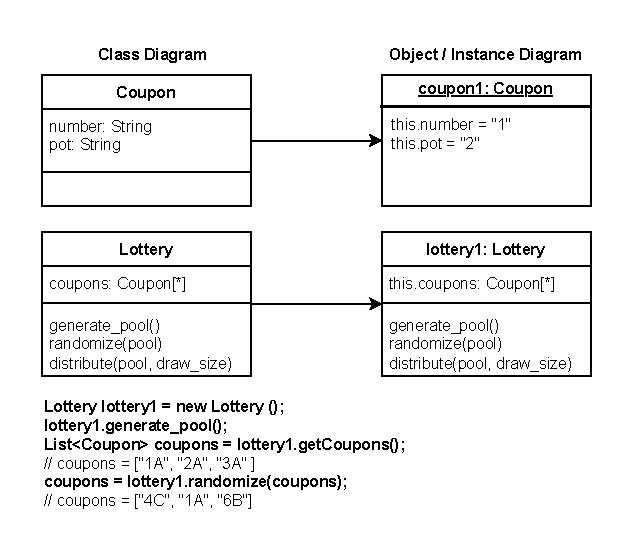
\includegraphics[width=\textwidth]{../assets/object-oriented.pdf}
	\caption{Pada gambar di atas metode \texttt{generate\_pool} menginisialisasi \texttt{coupons} pada objek \texttt{lottery1} dan \texttt{randomize} mengubah \textit{state} dari \texttt{coupons}.}
	\label{fig:ilustrasi-oop}
\end{figure}

\subsection{Pemrograman Berorientasi Objek (OOP)}
OOP menekankan pada pembuatan objek yang merupakan representasi dari entitas dunia nyata. Objek-objek ini memiliki \textbf{atribut} (data) dan \textbf{metode} (fungsi) yang mengoperasikan data tersebut. Salah satu karakteristik utama dari OOP adalah bahwa \textbf{objek dapat mengubah state-nya}, yakni nilai dari atribut-atribut yang dimilikinya bisa berubah selama program berjalan. Misalnya, pada Gambar \ref{fig:ilustrasi-oop}, metode \texttt{generate\_pool} menginisialisasi \texttt{coupons} pada objek \texttt{lottery1} dan \texttt{randomize} mengubah \textit{state} dari \texttt{coupons}. Beberapa konsep utama dalam OOP adalah:
\begin{itemize}
	\item \textbf{Kelas dan Objek}: Kelas adalah cetak biru dari objek. Objek adalah instansiasi dari kelas.
	\item \textbf{Enkapsulasi}: Pengelompokan data dan fungsi dalam objek, memungkinkan kontrol akses terhadap data.
	\item \textbf{Pewarisan}: Mekanisme untuk membuat kelas baru berdasarkan kelas yang sudah ada, mewarisi atribut dan metode.
	\item \textbf{Polimorfisme}: Kemampuan objek untuk diperlakukan sebagai bentuk lain dari objek yang berbeda, memungkinkan metode yang sama digunakan untuk tipe objek yang berbeda.
\end{itemize}


\begin{figure}[h]
	\centering
	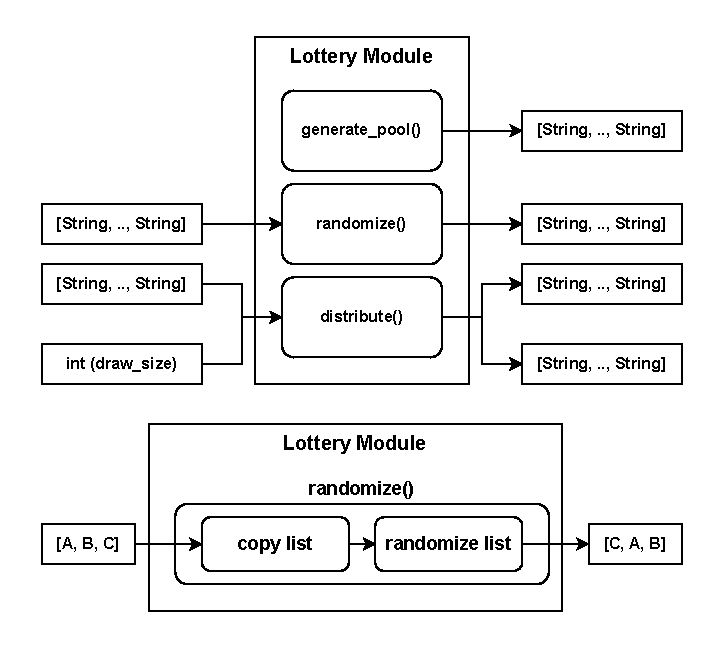
\includegraphics[width=\textwidth]{../assets/functional.pdf}
	\caption{Pada gambar di atas, \texttt{coupons = [A, B, C]} digandakan terlebih dahulu (\texttt{copy list}), kemudian diacak (\texttt{randomize list}) menghasilkan \texttt{coupons = [C, A, B]}. }
	\label{fig:contoh-fp}
\end{figure}

\subsection{Pemrograman Fungsional (FP)}
Pemrograman fungsional didasarkan pada konsep \textbf{fungsi matematika} yang tidak memiliki efek samping, sehingga fungsi akan selalu memberikan hasil yang sama untuk input yang sama. \textbf{FP tidak mengubah state dari nilai}, melainkan setiap operasi pada data menghasilkan \textbf{salinan baru} dari data tersebut dengan modifikasi yang diinginkan. Sebagai contoh, Pada Gambar \ref{fig:contoh-fp}, \texttt{coupons = [A, B, C]} digandakan terlebih dahulu (\texttt{copy list}), kemudian diacak (\texttt{randomize list}) menghasilkan \texttt{coupons = [C, A, B]}. Beberapa konsep kunci dari FP adalah:
\begin{itemize}
	\item \textbf{Fungsi Murni}: Fungsi yang tidak memodifikasi keadaan luar dan selalu memberikan hasil yang sama untuk argumen yang sama.
	\item \textbf{Immutability}: Data tidak dapat diubah setelah didefinisikan, yang meningkatkan prediktabilitas program. Setiap modifikasi menghasilkan salinan baru dari data.
	\item \textbf{Rekursi}: Pengulangan dilakukan melalui pemanggilan fungsi yang berulang, bukan melalui loop imperatif.
	\item \textbf{First-Class Functions}: Fungsi diperlakukan sebagai nilai yang dapat diteruskan sebagai parameter, dikembalikan sebagai hasil, atau disimpan dalam variabel.
\end{itemize}
Pemrograman fungsional lebih fokus pada transformasi data dengan fungsi, tanpa mengubah data secara langsung, sehingga mengurangi bug yang disebabkan oleh efek samping dan membuat program lebih mudah diuji.

\subsection{Perbandingan OOP dan FP}
\begin{itemize}
	\item OOP menekankan pada objek yang menyimpan state dan metode yang mengubah state tersebut, sedangkan FP menekankan pada fungsi murni yang \textbf{tidak mengubah state} melainkan \textbf{menghasilkan salinan baru} dari data sebagai hasil transformasi.
	\item Pada OOP, perubahan state adalah hal umum, sementara pada FP, data bersifat immutable, dan perubahan dihasilkan dengan mengkopi nilai input dan memodifikasinya.
	\item OOP biasanya menggunakan loop imperatif untuk iterasi, sementara FP menggunakan rekursi dan fungsi seperti \texttt{map}, \texttt{filter}, dan \texttt{reduce}.
	\item OOP lebih cocok untuk sistem yang melibatkan interaksi antar entitas (seperti GUI atau game), sedangkan FP lebih efisien untuk perhitungan matematis dan manipulasi data.
\end{itemize}

Kedua paradigma ini dapat saling melengkapi dan sering digunakan secara bersamaan dalam berbagai bahasa pemrograman modern.


\section{Menjalankan dan Menguji Kode dengan IEx}

IEx (Interactive Elixir) merupakan REPL (\textit{Read--Eval--Print Loop}) bawaan Elixir yang memungkinkan pengembang untuk langsung mencoba potongan kode, mengevaluasi fungsi, serta melakukan eksplorasi tanpa harus membuat file secara terpisah. Hal ini sangat membantu dalam proses belajar maupun pengujian cepat.

\subsection{Memulai IEx}
Untuk membuka sesi IEx, jalankan perintah berikut pada terminal:

\begin{lstlisting}[language=Elixir]
	$ iex
\end{lstlisting}

Jika berhasil, Anda akan masuk ke lingkungan interaktif dengan prompt seperti:

\begin{lstlisting}[language=Elixir]
	Interactive Elixir (1.16.0) - press Ctrl+C to exit
	iex(1)>
\end{lstlisting}

\subsection{Menjalankan Ekspresi Sederhana}
Anda dapat langsung menuliskan ekspresi atau fungsi bawaan Elixir. Contoh:

\begin{lstlisting}[language=Elixir]
	iex(1)> 1 + 2 * 3
	7
	
	iex(2)> String.upcase("hello world")
	"HELLO WORLD"
\end{lstlisting}

\subsection{Menguji Fungsi Buatan Sendiri}
Jika memiliki modul Elixir di dalam file, misalnya `hello.exs`:

\begin{lstlisting}[language=Elixir]
	defmodule Hello do
	def greet(name) do
	"Hello, #{name}!"
	end
	end
\end{lstlisting}

Maka Anda dapat memuat dan menguji fungsi tersebut di IEx:

\begin{lstlisting}[language=Elixir]
	iex(1)> c("hello.exs")
	[Hello]
	
	iex(2)> Hello.greet("Alice")
	"Hello, Alice!"
\end{lstlisting}

\subsection{Membuat Proyek Elixir dengan Mix}

Mix adalah build tool bawaan Elixir yang digunakan untuk membuat, mengelola, dan menjalankan proyek Elixir. Dengan Mix, pengembang dapat dengan mudah membuat struktur proyek, menambahkan dependensi, menjalankan test, serta membangun aplikasi.

Untuk membuat proyek baru, jalankan perintah berikut di terminal:

\begin{lstlisting}[language=Elixir]
	$ mix new nama_proyek
	$ cd nama_proyek
\end{lstlisting}

Perintah pertama membuat direktori proyek dengan struktur standar Elixir, sedangkan perintah kedua memindahkan Anda ke dalam direktori proyek tersebut.

\subsection{Menjalankan Script Sekaligus Masuk IEx}
Elixir juga mendukung menjalankan file dan langsung masuk ke mode interaktif menggunakan opsi `-S`:

\begin{lstlisting}[language=Elixir]
	$ iex -S mix
\end{lstlisting}

Perintah ini akan memuat proyek Mix yang sedang aktif sehingga modul dan dependensi dapat langsung digunakan dalam IEx.

\subsection{Ringkasan}
IEx menyediakan lingkungan praktis untuk:
\begin{enumerate}
	\item Mencoba ekspresi Elixir sederhana.
	\item Menguji fungsi buatan tanpa membuat aplikasi penuh.
	\item Mengeksplorasi modul, dokumentasi, dan debug.
\end{enumerate}
Dengan demikian, IEx merupakan alat yang esensial dalam pengembangan maupun pembelajaran Elixir.



\section{String di Elixir}

String adalah salah satu tipe data dasar di Elixir yang digunakan untuk merepresentasikan teks. String di Elixir didefinisikan dengan menggunakan tanda kutip ganda (\texttt{"..."}). Setiap string di Elixir adalah UTF-8 encoded binary, yang memungkinkan penggunaan karakter dari berbagai bahasa.

\subsection{Operasi Dasar pada String}

Elixir menyediakan berbagai operasi yang dapat dilakukan pada string, seperti menggabungkan, membandingkan, dan memanipulasi string. Beberapa operasi dasar termasuk:

\begin{itemize}
	\item \textbf{Penggabungan String}: Anda dapat menggabungkan dua atau lebih string menggunakan operator \texttt{<>}.
	\item \textbf{Interpolasi String}: Anda dapat menyisipkan nilai ekspresi atau variabel ke dalam string dengan menggunakan \texttt{\#\{...\}}.
	\item \textbf{Mengukur Panjang String}: Fungsi \texttt{String.length/1} dapat digunakan untuk mendapatkan jumlah karakter dalam string.
	\item \textbf{Mengubah Huruf Besar/Kecil}: Fungsi seperti \texttt{String.upcase/1} dan \texttt{String.downcase/1} digunakan untuk mengubah huruf string menjadi huruf besar atau kecil.
\end{itemize}

\subsection{Contoh Kode}

Berikut adalah beberapa contoh kode yang menunjukkan cara bekerja dengan string di Elixir:

\begin{lstlisting}[language=Elixir]
	# Menggabungkan dua string
	greeting = "Hello, " <> "world!"
	IO.puts(greeting)  # Output: Hello, world!
	
	# Interpolasi string
	name = "Elixir"
	message = "Welcome to #{name} programming!"
	IO.puts(message)  # Output: Welcome to Elixir programming!
	
	# Mengukur panjang string
	len = String.length("Hello")
	IO.puts(len)  # Output: 5
	
	# Mengubah string menjadi huruf besar
	IO.puts(String.upcase("elixir"))  # Output: ELIXIR
	
	# Mengubah string menjadi huruf kecil
	IO.puts(String.downcase("ELIXIR"))  # Output: elixir
\end{lstlisting}

Dalam contoh-contoh di atas, berbagai operasi dasar string seperti penggabungan, interpolasi, dan perubahan huruf besar/kecil diperlihatkan. Ini adalah beberapa contoh sederhana yang menunjukkan kekuatan dan fleksibilitas dalam bekerja dengan string di Elixir.

\section{List di Elixir}

List adalah salah satu tipe data utama di Elixir yang digunakan untuk menyimpan kumpulan elemen. List di Elixir diwakili oleh tanda kurung siku \texttt{[]} dan dapat menyimpan elemen-elemen dengan tipe data yang berbeda-beda, termasuk angka, string, dan bahkan list lainnya.

\subsection{Operasi Dasar pada List}

Elixir menyediakan berbagai operasi yang dapat dilakukan pada list, seperti menambahkan elemen, menggabungkan list, dan mengakses elemen tertentu. Beberapa operasi dasar termasuk:

\begin{itemize}
	\item \textbf{Menambah Elemen}: Anda dapat menambahkan elemen ke dalam list menggunakan operator kons \texttt{[head | tail]} atau dengan fungsi \texttt{List.insert\_at/3}.
	\item \textbf{Menggabungkan List}: Dua atau lebih list dapat digabungkan menggunakan operator \texttt{++}.
	\item \textbf{Mengakses Elemen}: Elemen dalam list dapat diakses dengan menggunakan notasi indeks atau dengan pola pencocokan (pattern matching).
	\item \textbf{Menghitung Panjang List}: Fungsi \texttt{length/1} digunakan untuk mendapatkan jumlah elemen dalam list.
	\item \textbf{Mencari Elemen dalam List}: Fungsi seperti \texttt{Enum.member?/2} digunakan untuk memeriksa apakah sebuah elemen ada dalam list.
\end{itemize}

\subsection{Contoh Kode}

Berikut adalah beberapa contoh kode yang menunjukkan cara bekerja dengan list di Elixir:

\begin{lstlisting}[language=Elixir]
	# Membuat list baru
	list = [1, 2, 3, 4, 5]
	IO.inspect(list)  # Output: [1, 2, 3, 4, 5]
	
	# Menambahkan elemen ke list
	new_list = [0 | list]
	IO.inspect(new_list)  # Output: [0, 1, 2, 3, 4, 5]
	
	# Menggabungkan dua list
	combined_list = [1, 2, 3] ++ [4, 5, 6]
	IO.inspect(combined_list)  # Output: [1, 2, 3, 4, 5, 6]
	
	# Mengakses elemen pertama dan sisa list
	[head | tail] = list
	IO.puts("Head: #{head}")  # Output: Head: 1
	IO.inspect(tail)          # Output: [2, 3, 4, 5]
	
	# Menghitung panjang list
	IO.puts("Length: #{length(list)}")  # Output: Length: 5
	
	# Memeriksa apakah sebuah elemen ada dalam list
	IO.puts(Enum.member?(list, 3))  # Output: true
\end{lstlisting}

Dalam contoh-contoh di atas, berbagai operasi dasar seperti menambah elemen, menggabungkan list, dan mengakses elemen diperlihatkan. List di Elixir sangat fleksibel dan banyak digunakan dalam pemrograman fungsional untuk menyimpan dan memanipulasi kumpulan data.

\section{Modul \texttt{Enum} di Elixir}

Modul \texttt{Enum} di Elixir menyediakan fungsi-fungsi untuk bekerja dengan koleksi data yang enumerable, seperti list, map, dan range. Fungsi-fungsi dalam modul \texttt{Enum} adalah sangat berguna untuk manipulasi dan transformasi data secara fungsional.

\subsection{Fungsi \texttt{Enum.shuffle/1}}

Fungsi \texttt{Enum.shuffle/1} digunakan untuk mengacak urutan elemen-elemen dalam sebuah list. Fungsi ini mengembalikan list baru dengan elemen-elemen yang telah diacak.

\begin{lstlisting}[language=Elixir]
	list = [1, 2, 3, 4, 5]
	shuffled_list = Enum.shuffle(list)
	IO.inspect(shuffled_list)  # Output: [3, 1, 4, 5, 2] (hasil acak)
\end{lstlisting}

\subsection{Fungsi \texttt{Enum.member?/2}}

Fungsi \texttt{Enum.member?/2} digunakan untuk memeriksa apakah sebuah elemen ada dalam koleksi enumerable. Fungsi ini mengembalikan \texttt{true} jika elemen ditemukan, dan \texttt{false} jika tidak.

\begin{lstlisting}[language=Elixir]
	list = [1, 2, 3, 4, 5]
	is_member = Enum.member?(list, 3)
	IO.puts(is_member)  # Output: true
\end{lstlisting}

\subsection{Fungsi \texttt{Enum.split/2}}

Fungsi \texttt{Enum.split/2} digunakan untuk membagi koleksi enumerable menjadi dua bagian berdasarkan jumlah elemen yang ditentukan. Fungsi ini mengembalikan tuple yang berisi dua list.

\begin{lstlisting}[language=Elixir]
	list = [1, 2, 3, 4, 5]
	{first_part, second_part} = Enum.split(list, 2)
	IO.inspect(first_part)   # Output: [1, 2]
	IO.inspect(second_part)  # Output: [3, 4, 5]
\end{lstlisting}

\subsection{Fungsi \texttt{Enum.map/2}}

Fungsi \texttt{Enum.map/2} menerapkan fungsi yang diberikan kepada setiap elemen dalam koleksi enumerable, menghasilkan koleksi baru dengan hasil-hasil tersebut.

\begin{lstlisting}[language=Elixir]
	list = [1, 2, 3, 4, 5]
	squared_list = Enum.map(list, fn x -> x * x end)
	IO.inspect(squared_list)  # Output: [1, 4, 9, 16, 25]
\end{lstlisting}

\subsection{Fungsi \texttt{Enum.filter/2}}

Fungsi \texttt{Enum.filter/2} memilih elemen-elemen dari koleksi enumerable yang memenuhi kondisi yang ditentukan oleh fungsi yang diberikan. Hasilnya adalah koleksi baru dengan elemen-elemen yang memenuhi syarat.

\begin{lstlisting}[language=Elixir]
	list = [1, 2, 3, 4, 5]
	even_numbers = Enum.filter(list, fn x -> rem(x, 2) == 0 end)
	IO.inspect(even_numbers)  # Output: [2, 4]
\end{lstlisting}

\subsection{Fungsi \texttt{Enum.reduce/3}}

Fungsi \texttt{Enum.reduce/3} secara berulang menerapkan fungsi yang diberikan kepada elemen-elemen dalam koleksi, mengakumulasi hasilnya. Fungsi ini sering digunakan untuk agregasi nilai-nilai.

\begin{lstlisting}[language=Elixir]
	list = [1, 2, 3, 4, 5]
	sum = Enum.reduce(list, 0, fn x, acc -> x + acc end)
	IO.puts(sum)  # Output: 15
\end{lstlisting}

Modul \texttt{Enum} sangat berguna untuk memanipulasi dan bekerja dengan koleksi data di Elixir. Dengan menggunakan fungsi-fungsi seperti \texttt{Enum.shuffle/1}, \texttt{Enum.member?/2}, \texttt{Enum.split/2}, \texttt{Enum.map/2}, \texttt{Enum.filter/2}, dan \texttt{Enum.reduce/3}, Anda dapat melakukan berbagai operasi pada data dengan cara yang efisien dan ekspresif.

\section{Pengulangan dengan \texttt{for} di Elixir}

Elixir menyediakan cara yang sangat elegan dan sederhana untuk melakukan pengulangan dengan menggunakan `for` loop. `for` loop di Elixir dapat digunakan untuk mengiterasi elemen-elemen dalam sebuah list, map, atau struktur lainnya. Selain itu, `for` loop juga dapat digunakan untuk nested looping, yaitu pengulangan bersarang.

\subsection{Single Looping}

Pengulangan tunggal menggunakan `for` di Elixir cukup mudah. Sebagai contoh, kita ingin mengiterasi sebuah list angka dan mengalikan setiap angkanya dengan 2.

\begin{lstlisting}[language=Elixir]
	numbers = [1, 2, 3, 4, 5]
	
	doubled_numbers = for n <- numbers do
	n * 2
	end
	
	IO.inspect(doubled_numbers)
	# Output: [2, 4, 6, 8, 10]
\end{lstlisting}

Dalam contoh di atas, `for n <- numbers` akan mengiterasi setiap elemen dalam list `numbers`, kemudian `n * 2` akan mengalikan setiap elemen dengan 2, dan hasilnya disimpan dalam list baru `doubled\_numbers`.

\subsection{Nested Looping}

`for` loop juga bisa digunakan untuk melakukan pengulangan bersarang (nested loop). Sebagai contoh, kita dapat membuat kombinasi dari dua list yang berbeda.

\begin{lstlisting}[language=Elixir]
	colors = ["red", "green", "blue"]
	shapes = ["circle", "square"]
	
	combinations = for color <- colors, shape <- shapes do
	{color, shape}
	end
	
	IO.inspect(combinations)
	# Output: [{"red", "circle"}, {"red", "square"}, {"green", "circle"}, {"green", "square"}, {"blue", "circle"}, {"blue", "square"}]
\end{lstlisting}

Dalam contoh di atas, `for color <- colors, shape <- shapes` akan mengiterasi setiap elemen dari list `colors` dan `shapes` untuk menghasilkan semua kombinasi yang mungkin antara warna dan bentuk. Hasilnya disimpan dalam list `combinations`.

Dengan `for` loop, Elixir menawarkan cara yang kuat dan fleksibel untuk mengelola pengulangan, baik untuk kasus tunggal maupun yang lebih kompleks seperti pengulangan bersarang.

\section{The Lottery Module}

Modul \texttt{Lottery} menyediakan fungsionalitas untuk mengelola sistem undian. Modul ini mencakup fungsi-fungsi untuk membuat, mengacak, memeriksa angka, dan mendistribusikan angka dalam pool undian. Berikut adalah kode lengkap untuk modul \texttt{Lottery}.

\begin{lstlisting}[language=elixir, caption={Complete Lottery Module}]
	defmodule Lottery do
	@moduledoc """
	This module provides functionalities for managing a lottery system.
	It includes functions for creating, shuffling, checking for numbers, and distributing numbers within the lottery pool.
	"""
	
	@spec greet() :: <<_::80>>
	@doc """
	Returns a greeting message.
	
	## Examples
	
	iex> Lottery.greet()
	"Good luck!"
	"""
	def greet do
	"Good luck!"
	end
	
	@spec generate_pool() :: [<<_::24, _::_*16>>, ...]
	@doc """
	Generates a pool of lottery numbers with different pots.
	
	## Returns
	
	- A list of lottery numbers with their respective pot numbers.
	
	## Examples
	
	iex> Lottery.generate_pool()
	["Number 1 in Pot 1", "Number 2 in Pot 1", ...]
	"""
	def generate_pool do
	numbers = ["Number 1", "Number 2", "Number 3", "Number 4", "Number 5", "Number 6"]
	pots = ["Pot 1", "Pot 2", "Pot 3", "Pot 4"]
	
	# Creates a pool by combining numbers and pots.
	for pot <- pots, number <- numbers do
	"#{number} in #{pot}"
	end
	end
	
	@doc """
	Randomizes the order of numbers in the pool.
	
	## Parameters
	
	- pool: The list of lottery numbers to be shuffled.
	
	## Returns
	
	- A new list with the numbers shuffled.
	
	## Examples
	
	iex> Lottery.randomize(["Number 1 in Pot 1", "Number 2 in Pot 2"])
	["Number 2 in Pot 2", "Number 1 in Pot 1"]
	"""
	def randomize(pool) do
	Enum.shuffle(pool)
	end
	
	@spec contains?(any(), any()) :: boolean()
	@doc """
	Checks if a specific number is included in the pool.
	
	## Parameters
	
	- pool: The list of lottery numbers.
	- number: The number to check for.
	
	## Returns
	
	- `true` if the number is in the pool, otherwise `false`.
	
	## Examples
	
	iex> Lottery.contains?(["Number 1 in Pot 1"], "Number 1 in Pot 1")
	true
	"""
	def contains?(pool, number) do
	Enum.member?(pool, number)
	end
	
	@doc """
	Distributes the pool into two parts based on the specified draw size.
	
	## Parameters
	
	- pool: The list of lottery numbers to be split.
	- draw_size: The number of numbers to include in the first part.
	
	## Returns
	
	- A tuple with two lists: the first list containing `draw_size` numbers, and the second list containing the remaining numbers.
	
	## Examples
	
	iex> Lottery.distribute(["Number 1 in Pot 1", "Number 2 in Pot 2"], 1)
	{["Number 1 in Pot 1"], ["Number 2 in Pot 2"]}
	"""
	def distribute(pool, draw_size) do
	Enum.split(pool, draw_size)
	end
	end
\end{lstlisting}

\section{Panduan Menjalankan Kode Elixir di Command Prompt}

Setelah Anda membuat modul \texttt{Lottery} seperti di atas, Anda dapat menjalankan dan menguji fungsinya menggunakan \texttt{iex} (Interactive Elixir) di command prompt. Berikut adalah langkah-langkahnya:

\subsection{Menggunakan \texttt{iex -S mix} dan Perintah \texttt{recompile}}

Perintah \texttt{iex -S mix} digunakan untuk memulai shell interaktif Elixir dan memuat konfigurasi serta dependensi proyek yang telah didefinisikan dalam file \texttt{mix.exs}. Dengan menggunakan perintah ini, Anda dapat:

\begin{itemize}
	\item Mengakses modul dan fungsi yang telah Anda buat dalam proyek Elixir.
	\item Menjalankan dan menguji kode Elixir secara interaktif.
	\item Memantau hasil dan output dari kode yang dijalankan dalam konteks proyek Anda.
\end{itemize}

\textbf{Contoh Penggunaan \texttt{iex -S mix}:}

1. **Buka Terminal atau Command Prompt** dan arahkan ke direktori proyek Elixir Anda.
2. **Jalankan perintah berikut** untuk memulai shell interaktif dengan konfigurasi proyek:
\begin{lstlisting}[language=bash]
	iex -S mix
\end{lstlisting}
3. **Gunakan Modul dan Fungsi** yang telah Anda definisikan dalam proyek.

Selain itu, selama pengembangan, Anda mungkin melakukan perubahan pada kode sumber. Untuk memuat ulang kode yang telah diubah tanpa keluar dari shell, Anda dapat menggunakan perintah `recompile`:

\textbf{Contoh Penggunaan \texttt{recompile}:}

1. Setelah memulai \texttt{iex -S mix}, lakukan perubahan pada kode sumber Anda.
2. Dalam shell \texttt{iex}, jalankan perintah berikut untuk mengkompilasi ulang kode:
\begin{lstlisting}[language=bash]
	recompile
\end{lstlisting}

Perintah ini akan mengkompilasi ulang file yang telah diubah dan memuat ulang modul yang bersangkutan, sehingga Anda dapat langsung melihat perubahan tanpa harus memulai ulang shell interaktif. 

Perintah \texttt{iex -S mix} dan \texttt{recompile} memudahkan pengembangan dan debugging dengan menyediakan lingkungan yang memungkinkan Anda untuk bereksperimen dan menguji kode dengan cepat.


\subsection{Menjalankan Kode di \texttt{iex}}

\begin{enumerate}
	\item Buka terminal atau command prompt.
	\item Navigasi ke direktori tempat file \texttt{lottery.ex} berada. Misalnya:
	\begin{lstlisting}[language=bash]
		cd path/to/your/project
	\end{lstlisting}
	\item Mulai sesi \texttt{iex} dengan perintah berikut:
	\begin{lstlisting}[language=bash]
		iex
	\end{lstlisting}
	\item Di dalam sesi \texttt{iex}, muat modul \texttt{Lottery} dengan perintah:
	\begin{lstlisting}[language=bash]
		c("lottery.ex") # atau path ke lottery.ex
	\end{lstlisting}
	\item Anda sekarang bisa memanggil fungsi-fungsi dalam modul \texttt{Lottery}. Misalnya:
	\begin{lstlisting}[language=bash]
		Lottery.greet()
		Lottery.generate_pool()
		Lottery.randomize(["Number 1 in Pot 1", "Number 2 in Pot 2"])
	\end{lstlisting}
\end{enumerate}

\subsection{Melakukan Reload Setelah Perubahan Kode}

Jika Anda mengubah kode di file \texttt{lottery.ex}, Anda perlu memuat ulang modul tersebut di \texttt{iex} untuk melihat perubahan. Berikut caranya:

\begin{enumerate}
	\item Simpan perubahan di file \texttt{lottery.ex}.
	\item Kembali ke sesi \texttt{iex} yang sedang berjalan.
	\item Muat ulang modul dengan perintah:
	\begin{lstlisting}[language=bash]
		r(Lottery)
	\end{lstlisting}
	\item Fungsi-fungsi dalam modul \texttt{Lottery} sekarang akan mencerminkan perubahan yang baru saja Anda buat.
\end{enumerate}

Dengan panduan ini, Anda dapat menjalankan dan menguji modul \texttt{Lottery} serta memperbaruinya secara interaktif di \texttt{iex}.


\section{Penjelasan Detail Modul Lottery}

\subsection{Definisi Modul}

Modul \texttt{Lottery} didefinisikan menggunakan kata kunci \texttt{defmodule}. Modul ini bertanggung jawab untuk mengelola sistem undian dan mencakup fungsi-fungsi untuk membuat, mengacak, memeriksa, dan mendistribusikan angka dalam pool undian.

\begin{lstlisting}[language=elixir, caption={Definisi Modul Lottery}]
	defmodule Lottery do
	@moduledoc """
	This module provides functionalities for managing a lottery system.
	It includes functions for creating, shuffling, checking for numbers, and distributing numbers within the lottery pool.
	"""
\end{lstlisting}

\subsection{Fungsi Salam}

Fungsi \texttt{greet/0} mengembalikan pesan salam sederhana. Fungsi ini merupakan contoh dasar dari fungsi tanpa parameter dan memiliki satu nilai balik.

\begin{lstlisting}[language=elixir, caption={Fungsi Salam}]
	@spec greet() :: <<_::80>>
	@doc """
	Returns a greeting message.
	
	## Examples
	
	iex> Lottery.greet()
	"Good luck!"
	"""
	def greet do
	"Good luck!"
	end
\end{lstlisting}

\subsection{Fungsi Pembentukan Pool}

Fungsi \texttt{generate\_pool/0} menghasilkan pool angka undian yang dikombinasikan dengan nomor pot. Fungsi ini mengembalikan daftar yang setiap angkanya dihubungkan dengan pot.

\begin{lstlisting}[language=elixir, caption={Fungsi Pembentukan Pool}]
	@spec generate_pool() :: [<<_::24, _::_*16>>, ...]
	@doc """
	Generates a pool of lottery numbers with different pots.
	
	## Returns
	
	- A list of lottery numbers with their respective pot numbers.
	
	## Examples
	
	iex> Lottery.generate_pool()
	["Number 1 in Pot 1", "Number 2 in Pot 1", ...]
	"""
	def generate_pool do
	numbers = ["Number 1", "Number 2", "Number 3", "Number 4", "Number 5", "Number 6"]
	pots = ["Pot 1", "Pot 2", "Pot 3", "Pot 4"]
	
	# Creates a pool by combining numbers and pots.
	for pot <- pots, number <- numbers do
	"#{number} in #{pot}"
	end
	end
\end{lstlisting}

\subsection{Fungsi Pengacakan}

Fungsi \texttt{randomize/1} menerima pool angka undian dan mengembalikan daftar baru dengan angka yang diacak. Fungsi ini menggunakan \texttt{Enum.shuffle/1} untuk mengacak urutan.

\begin{lstlisting}[language=elixir, caption={Fungsi Pengacakan}]
	@doc """
	Randomizes the order of numbers in the pool.
	
	## Parameters
	
	- pool: The list of lottery numbers to be shuffled.
	
	## Returns
	
	- A new list with the numbers shuffled.
	
	## Examples
	
	iex> Lottery.randomize(["Number 1 in Pot 1", "Number 2 in Pot 2"])
	["Number 2 in Pot 2", "Number 1 in Pot 1"]
	"""
	def randomize(pool) do
	Enum.shuffle(pool)
	end
\end{lstlisting}

\subsection{Fungsi Pemeriksaan Angka}

Fungsi \texttt{contains?/2} memeriksa apakah angka tertentu termasuk dalam pool. Fungsi ini mengembalikan \texttt{true} jika angka ditemukan dan \texttt{false} jika tidak.

\begin{lstlisting}[language=elixir, caption={Fungsi Pemeriksaan Angka}]
	@spec contains?(any(), any()) :: boolean()
	@doc """
	Checks if a specific number is included in the pool.
	
	## Parameters
	
	- pool: The list of lottery numbers.
	- number: The number to check for.
	
	## Returns
	
	- `true` if the number is in the pool, otherwise `false`.
	
	## Examples
	
	iex> Lottery.contains?(["Number 1 in Pot 1"], "Number 1 in Pot 1")
	true
	"""
	def contains?(pool, number) do
	Enum.member?(pool, number)
	end
\end{lstlisting}

\subsection{Fungsi Distribusi}

Fungsi \texttt{distribute/2} membagi pool menjadi dua bagian berdasarkan ukuran undian yang ditentukan. Fungsi ini mengembalikan tuple yang berisi dua daftar: satu dengan angka yang dipilih dan satu lagi dengan angka sisanya.

\begin{lstlisting}[language=elixir, caption={Fungsi Distribusi}]
	@doc """
	Distributes the pool into two parts based on the specified draw size.
	
	## Parameters
	
	- pool: The list of lottery numbers to be split.
	- draw_size: The number of numbers to include in the first part.
	
	## Returns
	
	- A tuple with two lists: the first list containing `draw_size` numbers, and the second list containing the remaining numbers.
	
	## Examples
	
	iex> Lottery.distribute(["Number 1 in Pot 1", "Number 2 in Pot 2"], 1)
	{["Number 1 in Pot 1"], ["Number 2 in Pot 2"]}
	"""
	def distribute(pool, draw_size) do
	Enum.split(pool, draw_size)
	end
\end{lstlisting}


\section{Latihan}

Bagian ini menyediakan latihan untuk memperdalam pemahaman mengenai String, List, modul `Enum`, serta pengulangan dengan `for` loop di Elixir. Selesaikan latihan di bawah ini dan uji kode yang Anda tulis di lingkungan `iex`.

\subsection{Latihan String}

Buatlah sebuah fungsi \texttt{greet\_person/1} yang menerima sebuah nama dalam bentuk string dan mengembalikan pesan sapaan seperti "Hello, [nama]!".

\begin{lstlisting}[language=Elixir]
	defmodule StringExercise do
	def greet_person(name) do
	"Hello, " <> name <> "!"
	end
	end
	
	# Contoh penggunaan:
	StringExercise.greet_person("Elixir")
	# Output: "Hello, Elixir!"
\end{lstlisting}

\subsection{Latihan List}

Buatlah sebuah fungsi \texttt{sum\_list/1} yang menerima sebuah list angka dan mengembalikan jumlah dari semua angka tersebut.

\begin{lstlisting}[language=Elixir]
	defmodule ListExercise do
	def sum_list(numbers) do
	Enum.sum(numbers)
	end
	end
	
	# Contoh penggunaan:
	ListExercise.sum_list([1, 2, 3, 4, 5])
	# Output: 15
\end{lstlisting}

\subsection{Latihan Modul \texttt{Enum}}

Gunakan fungsi \texttt{Enum.shuffle/1} untuk mengacak urutan elemen dalam sebuah list.

\begin{lstlisting}[language=Elixir]
	defmodule EnumExercise do
	def shuffle_list(list) do
	Enum.shuffle(list)
	end
	end
	
	# Contoh penggunaan:
	EnumExercise.shuffle_list([1, 2, 3, 4, 5])
	# Output: [3, 5, 1, 4, 2] (urutan dapat berbeda setiap kali)
\end{lstlisting}

\subsection{Latihan \texttt{for} Loop Tunggal}

Buatlah sebuah \texttt{for} loop yang mengiterasi angka dari 1 hingga 10 dan mencetak angka-angka tersebut.

\begin{lstlisting}[language=Elixir]
	for n <- 1..10 do
	IO.puts(n)
	end
	
	# Output:
	# 1
	# 2
	# 3
	# 4
	# 5
	# 6
	# 7
	# 8
	# 9
	# 10
\end{lstlisting}

\subsection{Latihan \texttt{for} Loop Bersarang}

Buatlah sebuah \texttt{for} loop bersarang yang menghasilkan semua pasangan karakter dari dua list huruf.


\begin{lstlisting}[language=Elixir]
	for letter1 <- ["A", "B", "C"], letter2 <- ["X", "Y", "Z"] do
	{letter1, letter2}
	end
	
	# Output:
	# [{"A", "X"}, {"A", "Y"}, {"A", "Z"}, {"B", "X"}, {"B", "Y"}, {"B", "Z"}, {"C", "X"}, {"C", "Y"}, {"C", "Z"}]
\end{lstlisting}

\subsection{Latihan Membuat Sistem Manajemen Inventaris}

Modul ini mengelola inventaris barang dengan fungsi-fungsi untuk menambahkan barang, menghapus barang, memeriksa ketersediaan barang, dan mendistribusikan barang ke berbagai lokasi.

\begin{lstlisting}[language=Elixir, caption={Modul Manajemen Inventaris}]
	defmodule Inventory do
	@moduledoc """
	Modul ini menyediakan fungsionalitas untuk mengelola sistem inventaris.
	Ini mencakup fungsi untuk menambahkan barang, menghapus barang, memeriksa ketersediaan barang, dan mendistribusikan barang ke lokasi yang berbeda.
	"""
	
	@spec add_item(String.t(), integer()) :: :ok
	@doc """
	Menambahkan barang baru ke inventaris.
	
	## Parameter
	
	- item: Nama barang.
	- quantity: Jumlah barang yang akan ditambahkan.
	
	## Examples
	
	iex> Inventory.add_item("Laptop", 10)
	:ok
	"""
	def add_item(item, quantity) do
	IO.puts("Menambahkan #{quantity} #{item} ke inventaris.")
	:ok
	end
	
	@spec remove_item(String.t(), integer()) :: :ok
	@doc """
	Menghapus barang dari inventaris.
	
	## Parameter
	
	- item: Nama barang.
	- quantity: Jumlah barang yang akan dihapus.
	
	## Examples
	
	iex> Inventory.remove_item("Laptop", 5)
	:ok
	"""
	def remove_item(item, quantity) do
	IO.puts("Menghapus #{quantity} #{item} dari inventaris.")
	:ok
	end
	
	@spec check_availability(String.t()) :: integer()
	@doc """
	Memeriksa ketersediaan barang dalam inventaris.
	
	## Parameter
	
	- item: Nama barang yang ingin diperiksa.
	
	## Returns
	
	- Jumlah barang yang tersedia.
	
	## Examples
	
	iex> Inventory.check_availability("Laptop")
	10
	"""
	def check_availability(item) do
	IO.puts("Memeriksa ketersediaan #{item}.")
	10
	end
	
	@spec distribute_items([String.t()], String.t()) :: :ok
	@doc """
	Mendistribusikan barang ke lokasi yang berbeda.
	
	## Parameter
	
	- items: Daftar barang yang akan didistribusikan.
	- location: Lokasi tujuan distribusi.
	
	## Examples
	
	iex> Inventory.distribute_items(["Laptop", "Mouse"], "Gudang A")
	:ok
	"""
	def distribute_items(items, location) do
	IO.puts("Mendistribusikan barang ke #{location}.")
	:ok
	end
	end
\end{lstlisting}

\subsection{Latihan Membuat Sistem Pendaftaran Kelas}

Modul ini mengelola pendaftaran siswa untuk kelas dengan fungsi-fungsi untuk mendaftar siswa, membatalkan pendaftaran, memeriksa pendaftaran, dan mengatur jadwal kelas.

\begin{lstlisting}[language=Elixir, caption={Modul Pendaftaran Kelas}]
	defmodule ClassRegistration do
	@moduledoc """
	Modul ini menyediakan fungsionalitas untuk mengelola sistem pendaftaran kelas.
	Ini mencakup fungsi untuk mendaftar siswa, membatalkan pendaftaran, memeriksa pendaftaran, dan mengatur jadwal kelas.
	"""
	
	@spec register_student(String.t(), String.t()) :: :ok
	@doc """
	Mendaftar siswa ke kelas.
	
	## Parameter
	
	- student: Nama siswa.
	- class: Nama kelas yang akan diikuti.
	
	## Examples
	
	iex> ClassRegistration.register_student("Alice", "Matematika")
	:ok
	"""
	def register_student(student, class) do
	IO.puts("Mendaftar #{student} ke kelas #{class}.")
	:ok
	end
	
	@spec cancel_registration(String.t(), String.t()) :: :ok
	@doc """
	Membatalkan pendaftaran siswa dari kelas.
	
	## Parameter
	
	- student: Nama siswa.
	- class: Nama kelas yang akan dibatalkan.
	
	## Examples
	
	iex> ClassRegistration.cancel_registration("Alice", "Matematika")
	:ok
	"""
	def cancel_registration(student, class) do
	IO.puts("Membatalkan pendaftaran #{student} dari kelas #{class}.")
	:ok
	end
	
	@spec check_registration(String.t()) :: [String.t()]
	@doc """
	Memeriksa kelas yang diikuti oleh siswa.
	
	## Parameter
	
	- student: Nama siswa yang ingin diperiksa.
	
	## Returns
	
	- Daftar kelas yang diikuti oleh siswa.
	
	## Examples
	
	iex> ClassRegistration.check_registration("Alice")
	["Matematika", "Fisika"]
	"""
	def check_registration(student) do
	IO.puts("Memeriksa pendaftaran untuk #{student}.")
	["Matematika", "Fisika"]
	end
	
	@spec schedule_class(String.t(), String.t()) :: :ok
	@doc """
	Mengatur jadwal untuk kelas.
	
	## Parameter
	
	- class: Nama kelas.
	- schedule: Jadwal kelas.
	
	## Examples
	
	iex> ClassRegistration.schedule_class("Matematika", "Senin, 09:00")
	:ok
	"""
	def schedule_class(class, schedule) do
	IO.puts("Mengatur jadwal kelas #{class} ke #{schedule}.")
	:ok
	end
	end
\end{lstlisting}


\section{Soal: Mengembangkan Sistem Kuis dalam Elixir}

Pada latihan ini, Anda diminta untuk membuat sebuah modul Elixir yang bernama \texttt{Quiz} dengan tujuan untuk mengelola sistem kuis. Modul ini harus memiliki fungsi-fungsi berikut:

\begin{enumerate}
	\item \texttt{generate\_questions/0}: Fungsi ini bertugas untuk menghasilkan daftar pertanyaan kuis. Setiap pertanyaan harus memiliki opsi jawaban yang berbeda-beda.
	
	\item \texttt{randomize\_questions/1}: Fungsi ini menerima daftar pertanyaan yang dihasilkan dari fungsi sebelumnya dan mengacak urutan pertanyaan tersebut.
	
	\item \texttt{check\_answer/3}: Fungsi ini bertugas untuk memeriksa apakah jawaban yang diberikan oleh peserta kuis sesuai dengan jawaban yang benar. Parameter yang diterima adalah daftar pertanyaan, jawaban peserta, dan jawaban yang benar.
	
	\item \texttt{score\_quiz/2}: Fungsi ini menerima daftar jawaban peserta dan daftar jawaban yang benar, kemudian menghitung skor akhir berdasarkan jumlah jawaban yang benar.
\end{enumerate}

\textbf{Tugas:} Implementasikan modul \texttt{Quiz} dalam bahasa Elixir, dan berikan contoh cara memanggil fungsi-fungsi tersebut di dalam \texttt{iex}.



